\documentclass[a4paper]{article}

\usepackage[T1]{fontenc}
\usepackage[utf8]{inputenc}
\usepackage[polish]{babel}
\usepackage{graphicx}
\graphicspath{{.}}

\usepackage[left = 2cm, right = 2cm, top = 2cm, bottom = 2cm] {geometry}

\usepackage{amsmath, amsfonts}
\usepackage{textcomp}

\pagestyle{empty}

\author{}
\title{}
\date{\today}

\begin{document}
\section*{Instrukcja gry "Monopoly UWr"}

%\paragraph*{Informacje ogólne}
\noindent \textbf{1. Informacje ogólne}\\
\noindent Gra przeznaczona jest dla 4 graczy. Mogą być nimi również zawarte w grze boty.
\vspace{10pt}

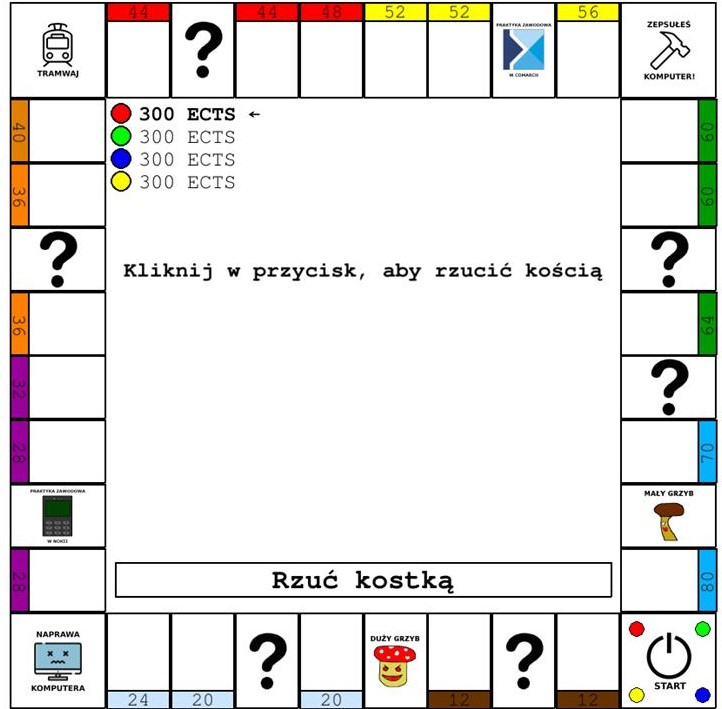
\includegraphics[scale=0.6]{board.png}

\noindent \textbf{2. Cel gry}\\
\noindent Celem jest zapisanie się i napisanie egzaminów z czterech przedmiotów lub doprowadzenie pozostałych graczy do utraty wszystkich punktów.
\vspace{10pt}

\noindent \textbf{3. Oznaczenia graczy}\\
\indent 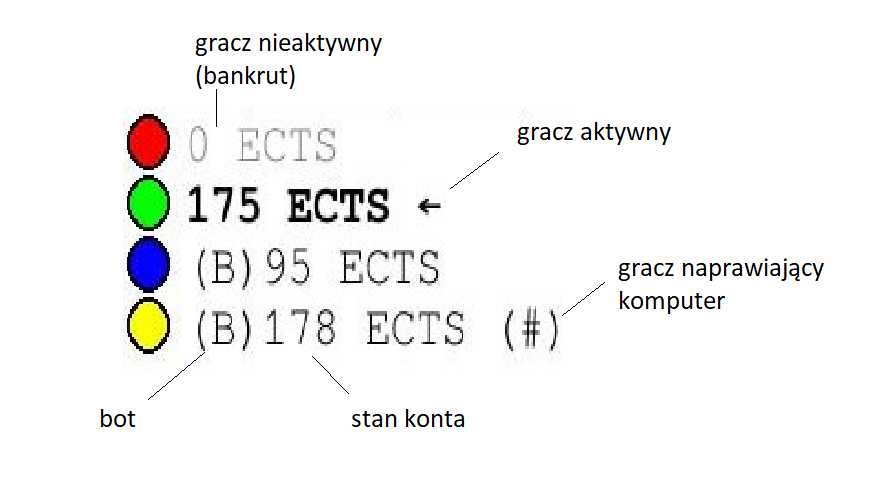
\includegraphics[scale=0.5]{ozn_graczy.png}

%\paragraph*{Rozgrywka}
\noindent \textbf{4. Rozgrywka}\\
\noindent Wszyscy gracze rozpoczynają rozgrywkę na polu 'start'. Pionki graczy reprezentowane są przez kolorowe kółka. Tura gracza składa się z następujących akcji:\\
- rzut dwiema kostkami,\\
\indent 
\includegraphics [scale=0.4]{kostki.png}\\
- przesunięcie swojego pionka o liczbę pól równą sumie wyrzuconych oczek w kierunku zgodnym z ruchem wskazówek zegara,\\
- wykonanie instrukcji zgodnie z opisem pola, na który został przesunięty pionek,\\
- zakończenie tury.\\
W przypadku wyrzucenia dubletu:\\
\indent 
\includegraphics[scale=0.4]{dublet.png}\\
(czyli takiej samej ilości oczek na obydwu kostkach), gracz przesuwa pionek o sumę oczek na kostkach i rzuca ponownie kośćmi. Jeśli trzy razy pod rząd wypadnie graczowi dublet, jego pionek jest przesuwany na pole 'naprawa komputera' (patrz: Plansza i pola). 
\vspace{10pt}

%\paragraph*{Waluta}
\noindent \textbf{5. Waluta}\\
\noindent Każdy gracz otrzymuje na starcie 300 punktów ECTS. Po każdorazowym przejściu lub stanięciu na polu 'start' gracz otrzymuje 30 ECTS.
\vspace{10pt}

%\paragraph*{Plansza}
\noindent \textbf{6. Plansza i pola}\\
Plansza składa się z 36 pól. Wyróżniamy wśród nich:\\
\noindent \textbf{a) start} - początek rozgrywki.\\ 
\indent
\includegraphics[scale=0.6]{start.png}\\
\indent Po każdym przejściu przez to pole, dostajemy dodatkowe 30 ECTS.\\

\noindent \textbf{b) zakłady} - jest ich 8.\\
\noindent Każdy zakład składa się z dwóch lub trzech pól przedmiotów, oznaczonych tym samym kolorem.\\

\noindent \textbf{c) pola przedmiotów} - są 22 takie pola, oznaczone kolorowym paskiem wraz z ceną nabycia.\\
\indent 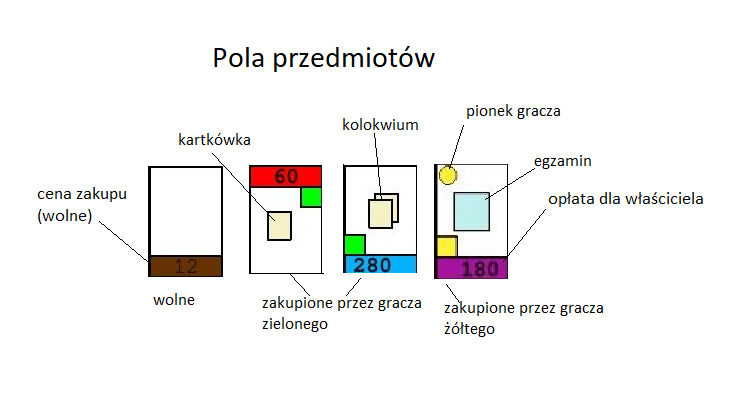
\includegraphics[scale=0.8]{pola.png}\\
\noindent Każde takie pole reprezentuje jeden z wykładanych w instytucie przedmiotów. Można zapisać się na niego poprzez oddanie punktów ECTS w ilości przypisanej do danego pola (oczywiście jeśli gracz ma na to środki). Zapisanie gracza na dany przedmiot jest oznaczane kwadratem w kolorze pionka gracza. Aby zaliczyć dany przedmiot, trzeba napisać z niego odpowiednio kartkówkę, kolokwium i egzamin - każda taka operacja kosztuje pewną przypisaną ilość ECTS. Prace pisemne można pisać jedynie na przedmiocie, na który gracz jest zapisany. Przedmiot uznaje się za zaliczony, jeśli gracz napisał z niego egzamin. Uwaga - za jednym razem można wykonać tylko jedną z tych czynności. Jeśli gracz stanie na przedmiocie, na który zapisał się już ktoś inny, oddaje tej osobie ilość ECTS przypisaną do danego pola. Można również zastąpić aktualnego posiadacza pola - kosztuje to tyle, ile wynosi aktualna wartość pola, powiększona o 100\%. Uwaga - nowy gracz zapisany na przedmiot zaczyna go od początku - musi sam od początku napisać wszystkie prace pisemne.\\ 

\noindent \textbf{d) mały grzyb} - jest jedno takie pole.\\
\indent 
\includegraphics[scale=0.5]{s_mush.png}\\
\noindent Stanięcie na nim skutkuje utratą 15 punktów ECTS.\\

\noindent \textbf{e) duży grzyb} - jest jedno takie pole.\\
\indent 
\includegraphics[scale=0.5]{l_mush.png}\\
\noindent Stanięcie na nim skutkuje utratą 30 punktów ECTS.\\

\noindent \textbf{f) szansa} - jest 6 takich pól, oznaczonych znakiem zapytania.\\
\indent 
\includegraphics[scale=0.7]{chance.png}\\
\noindent Po stanięcu na nim losuje się karta, która wskazuje, jaka akcja się wykona. Nie ma możliwości uniknięcia wylosowanej czynności.\\

\noindent \textbf{g) tramwaj} - pole umożliwiające przejście do wybranego przez siebie innego pola.\\
\indent
\includegraphics[scale=0.8]{tram.png}\\
\noindent Gracz może przejść tylko na pole, które posiada lub które nie zostało jeszcze zakupione lub na pole specjalne z wyjątkiem pola tramwaju i zajętych pól praktyk. \\

\noindent \textbf{h) zepsułeś komputer} - pole, które automatycznie przenosi gracza na pole naprawa komputera, gdzie musi pozostać 3 tury lub opuścić je w inny sposób.\\
\indent
\includegraphics[scale=0.8]{jail.png}\\
\noindent \textbf{i) naprawa komputera} - jeśli gracz stanie na tym polu, musi pozostać na nim przez 2 tury, zanim będzie mógł je opuścić. Innym sposobem na opuszczenie tego pola jest oddanie 30 ECTS lub wylosowanie na dwóch kostkach dubletu.\\

\indent
\includegraphics[scale=0.8]{injail.png}\\
\noindent \textbf{j) praktyki} - są 2 takie pola.\\
\noindent Aby się na nie zapisać, trzeba oddać przypisaną ilość punktów ECTS. Wykup praktyk jest obowiązkowy i kosztuje 45 ECTS. Praktyk nie można przejąć od kogoś - kto pierwszy, ten lepszy. Gracz, który stanie na polu praktyk należącym do innego gracza musi oddać posiadaczowi pola 20 ECTS.
\vspace{10pt}

%\paragraph*{7.Co, jeśli staniemy na polu i nie stać na na opłacenie akcji związanej z nim?}
\noindent \textbf{7. Co, jeśli gracz stanie na polu i nie stać go na opłacenie akcji z nim związanej?}\\
\noindent Gracz bankrutuje, oddaje wszystkie swoje pola do puli dostępnych pól i kończy grę.
\vspace{10pt}

\noindent Dobór nazw przedmiotów i ich pozycji na planszy jest losowy, niekierowany naszymi preferencjami.
\end{document}


